
El CNC es una nueva estrategia de reconocimiento de gestos basada en redes neuronales competitivas. El CNC utiliza múltiples clasificadores internos del mismo tipo entrenados en paralelo, y para clasificar integra los resultados de estos clasificadores mediante un proceso de decisión para añadir robustez al proceso de reconocimiento y aumentar la tasa de aciertos. La estructura de un CNC con $p$ subclasificadores se muestra en la figura \ref{fig:cnc}.

\begin{figure}
\centering
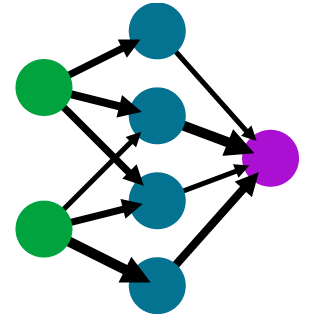
\includegraphics[scale = 0.5]{img/cnc}
\caption{a) CNC Architecture b) Subclassifier module}
\label{fig:cnc}
\end{figure}

\subsubsection{Classifier structure and functioning}

When a sample $\ve{s}$ enters the classifier, the Splitter module generates the sequence of basic components $\ve{bc}$ and sends a copy to each of the $p$ subclassifiers. Note that each basic component $\ve{bc}[j]$ is simply the cartesian or angle representation of the $jth$ direction vector described in the previous section. The Competitive Feature Encoder Module (CFEM ) in each subclassifier (figure \ref{fig:cnc} b) implements a neural network $nn'$ with $m$ neurons $h_1', h_2', \dots ,h_m'$, trained with the well-known CPN learning algorithm \cite{hecht1987counterpropagation}. Given a sequence of $n$ basic components (a sample), the CFEM maps it into a characteristic vector $\ve{v'}$ according to:

\begin{alignat*}{2}
\ve{v'} &=(v_1', v_2',\dots, v_m' ) \\
v_k'&= count(h_k') / n & k=1..m
\end{alignat*}
 
where $count(h_k')$ represents the number of basic components for which the neuron $h_k'$ had an activation value greater than other neurons. Therefore, $\ve{v'}$ codes information about the distribution of each basic component of the sample $\ve{s}$ according to the hidden space. Since the $nn's$ are trained independently, each will produce a classification based on different clusterings, hopefully complementary to each other.

The Competitive Evaluator Module (CEM) contains a neural network $nn$ with a competitive layer composed of $z$ hidden neurons $h_1,\dots,h_{z}$ with corresponding weights $\ve{w_1},\dots,\ve{w_{z}}$, where $z$ is determined by the learning algorithm. The neurons of this layer are stimulated with the vector $\ve{v'}$ to output a vector $\ve{v}=(v_1,\dots,v_{z})$ of scores. The network deviates from the typical competitive architecture in that instead of identifying a unique winner neuron, this vector represents the degree of membership of the sample to each neuron using the inverse of the Manhattan distance $||\cdot||$ as a similarity function, and is given by $ v_k&= 1/ ||(\ve{v'},\ve{w_k})|| & k=1..z $.
  

Each neuron $h_k$ is associated with a gesture class $c$ by means of a function $f::Neuron->Class$, and therefore such scores $\ve{v}$ also represent the degree of membership of the sample to each class. Finally, the Integrator module receives the outputs $\ve{v_i}, \quad i=1..p$ of every classifier, and calculates the corresponding class as $class=f(max_k(scores))$, where $scores=\sum_{i=1}^{p} \ve{v_i}$ and $max_k$ returns the index of the vector component (hidden neuron) with the maximum value.

\subsubsection{Learning algorithm}

The subclassifiers are trained independently in two stages. First, the $nn'$ of each CFEM is trained with the classical CPN iterative learning algorithm using the basic components of all samples and the Manhattan distance as a similarity function.

After the CFEM's training is finished, each $h_i'$ corresponds to the centroid of a cluster of basic components. Given the nontraditional use of each $nn'$ in the generation of characteristic vectors $\ve{v}'$on the training algorithm can be stopped very quickly (as early as two iterations in our tests) while still obtaining good results.

The neural network $nn$ of the CEM requires no training. Once the CFEM's training is complete, the $nn$ is built with $z = |C| \times u$ neurons $h_i$, where $u$ is the number of samples of each class and $|C|$ the number of classes.  To each $h_i$ corresponds a weight vector $\ve{w_i}=\ve{v_i'}$ where $\ve{v_i'}$ is the characteristic vector generated by the CFEM when presented with the basic components of sample $\ve{s_{i}}$. The mapping function $f$ is simply $f(i)=c_i$, that is, given sample index $i$, it returns the class label of sample $i$. 